\chapter{Methods and Results}

\section{Assessing the impact of transfer learning}

There are no results available from SIGMORPHON that directly measure the impact of transfer learning while controlling for other model parameters. 

SIGMORPHON 2018 task 1 used a string transduction model as a baseline, and received a variety of submitted models which all used a neural component but many of which took advantage of ensembling with string transduction methods. It did not explicitly make transfer learning data available, though one team did use multilingual training data to build its model \parencite{Cotterell2018b}.

The goal of the SIGMORPHON 2019 task 1 was the same as SIGMORPHON 2018 - morphological inflection - but it was specifically a transfer learning task. For the source language, a high-resource data set was provided, and for the target language a low-resource data set; these data sets are identical in size and format to the 2018 high- and low-resource training sets, but they were resampled and so don't contain exactly the same data. SIGMORPHON 2019 provided four baseline models for task 1, all of which were purely neural and differed by attention mechanism, and all submissions were neural models \parencite{McCarthy2019}. 

Given the similarity of data and goals between SIGMORPHON 2018 and 2019, it may be surprising that, for 50 of the 100 training pairs, higher accuracy was achieved on the target language in low-resource settings by the best model of 2018 than by any submission in 2019. It might have been expected that with access to additional data, as well as information from the previous year about which models were successful, models in 2019 should have avoided declining performance. The reason for the performance declines may be that in 2018, the models that performed best in low-resource settings were actually quite different than those that scored well in high-resource settings. Models adapted to low-resource settings tended to avoid pure reliance on neural encoder-decoder models and used techniques such as using string transduction to learn edit sequences and string alignments, and biasing toward copying characters. With the task refocused on neural transfer learning in 2019, many of these techniques might have been dropped. It also may be the case that, since training sets were resampled from 2018 to 2019, the languages that saw worsened performance in 2019 simply had by random chance less useful training sets that year. The low-resource training sets in 2018 and 2019 were relatively small with at most 100 examples, making for greater likelihood of chance sampling effects (\cite{McCarthy2019}, \cite{Cotterell2018b}).

Despite the many confounding factors between the 2018 and 2019 best model performances, some suggestive results are yielded by comparing the best performance of any submission on each pair in 2019 to the best performance of any 2018 submission on the comparable task of modeling the pair's target language in a low-resource setting. Barring differences in modeling technique and data sampling, the two problems are essentially equivalent - using about 100 examples of a language to predict any other inflected form from that language - with the major difference being the transfer learning data, about 10,000 examples of a different language, that was made available in 2019. 

I looked at rudimentary typological, genealogical, and sampling metrics of the languages and training pairs to find correlations with model improvements between 2018 and 2019. The methods of generation of this data, and statistical analysis of it, are presented in this section; potential interpretations and implications are discussed in the next section.

\section{Genealogical distance}

SIGMORPHON 2019 stated that 20 of its 100 language pairs were distantly or unrelated, based on the language "family" designations in SIGMORPHON 2018. I used the Ethnologue language genealogy designations to generate a three-tiered distance designation: "Closely related" (in the same language family and subfamily), "Distantly related" (in different subfamilies of the same family), and "Unrelated" (in different families). By my designation, there are 62 closely related pairs, 31 distantly related pairs, and 7 unrelated pairs.

I conjecture that most distantly related pairs have dissimilar enough forms as to behave much more like unrelated languages with perhaps coincidental structural similarities than like closely related languages. However, my designations are not a fine-grained or necessarily consistent metric of actual similarity; some language families are much more internally diverse than others, and subfamily divisions were chosen somewhat arbitrarily. 

On average, more distantly related language pairs actually perform better and show more improvement between 2018 and 2019, perhaps suggesting that transfer learning between closely related languages confuses the model, although this result is not statistically significant.

\begin{figure}[ht]
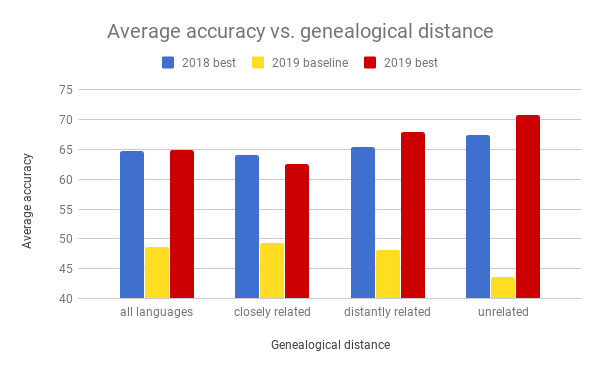
\includegraphics[width=12cm]{images/Average_accuracy_vs_genealogical_distance.png}
\centering
\end{figure}

I conducted all statistical tests on both the set of all language pairs and the set of all distantly related and unrelated language pairs, but no statistically significant results were achieved over the set of all language pairs; perhaps because genealogical relationship is too strong a confounding variable.

\section{Part of speech category overlap}

As discussed in the data section, the UniMorph annotations in the training data were scraped to discover the full set of morphological categories for which each part of speech could be inflected in each language. These category sets were used to generate a metric of structural similarity I call category overlap.

\subsection{Calculating overlap}

For each part speech in each of two languages, given the category sets $C_{POS, language\ A}$ and $C_{POS, language\ B}$, the overlap was calculated as

\[overlap(POS, language\ A, language\ B) = \frac{\abs*{C_{POS, language\ A}\ \cap\ C_{POS, language\ B}}}{\abs*{C_{POS, language\ A}\ \cup\ C_{POS, language\ B}}}\]

Take as an example the category overlap of nouns in German and Greek. The German category set for nouns is $C_{N,German} = \{ACC, DAT, GEN, NOM, PL, SG\}$ - German inflects nouns for singular and plural number and four grammatical cases. The Greek nominal category set is similar, except that it lacks a dative case and has a vocative case: $C_{N,Greek} = \{ACC, VOC, GEN, NOM, PL, SG\}$. The nominal category overlap is 

$overlap(N, German, Greek)$\\
$= \frac{\abs*{\{ACC, DAT, GEN, NOM, PL, SG\}\ \cap\ \{ACC, VOC, GEN, NOM, PL, SG\}}}{\abs*{\{ACC, DAT, GEN, NOM, PL, SG\}\ \cup\ \{ACC, VOC, GEN, NOM, PL, SG\}}}$\\
$= \frac{\abs*{\{ACC, GEN, NOM, PL, SG\}}}{\abs*{\{ACC, DAT, VOC, GEN, NOM, PL, SG\}}}$\\
$= \frac{5}{7} \approx .71$\\

It is not uncommon for one or both languages in a pair to lack any morphological categories for a particular part of speech; many languages do not have training data for all parts of speech. If only one language has an empty tagset for a part of speech, then by the above formula the category overlap is 0. If both languages have empty tagsets, the above formula would yield $\frac{0}{0}$, not a real number; in such a case the pair is excluded from analysis, which is why $n$ is less than the total number of language pairs in the findings below.

\subsection{Correlation with model performance}

Overall, verbal category overlap was much more predictive than nominal category overlap of performance changes between 2018 and 2019. In particular, the verbal category overlap of a transfer learning pair had a highly significant (p<.01) relationship with year over year accuracy improvement, with an additional .1 verbal category overlap score predicting a 3.7\% jump in absolute model accuracy between the two years. The relationship of nominal category overlap to model improvement did not rise to any significance threshold.

\begin{figure}[ht]
\includegraphics[width=12cm]{images/generated/significant/Accuracy_Improvement_vs_2018_vs_V_category_overlap_distantly_related_and_unrelated_language_pairs.png}
\centering
\caption{The relationship between a pair's verbal category overlap and the best team's performance in 2019 relative to 2018.}
\end{figure}

\begin{figure}[ht]
\includegraphics[width=12cm]{images/generated/insignificant/Accuracy_Improvement_vs_2018_vs_N_category_overlap_distantly_related_and_unrelated_language_pairs.png}
\centering
\caption{The relationship between a pair's nominal category overlap and the best team's performance in 2019 relative to 2018.}
\end{figure}

I used randomized permutation testing to approximate the significance level of the correlation.

\section{Part of speech distribution similarity}

The UniMorph tags identify four broad parts of speech cross-linguistically in the SIGMORPHON data: nouns, verbs, adjectives, and determiners. However, there is only one language among the 79 in the SIGMORPHON 2019 data that has all of these parts of speech represented; 64 languages have verb data, 55 have noun data, 40 have adjective data, and only 2 have determiner data. 

I use similarity between the relative distributions of parts of speech in source and target training sets as a metric of data set similarity. Part of speech distribution in the SIGMORPHON data is not necessarily an indication of actual linguistic typology; while some languages lack inflection on some parts of speech, there are also omissions in the SIGMORPHON data due to data sparsity \parencite{Cotterell2018b}.

\subsection{Calculating similarity}

My part of speech distribution similarity statistic is simply the statistical distance between the part of speech distributions of the two languages, calculated by summing the differences of the proportions of each part of speech between the two languages. That is, if $f_{POS, language}$ is the number of training forms for a given language and part of speech and $f_{language}$ is the total number of training forms for a language, the part of speech distribution similarity between language A and language B is

\[POSDS(language\ A, language\ B) = \sum\limits_{POS}\ \abs*{\frac{f_{POS, language\ A}}{f_{language\ A}} - \frac{f_{POS, language\ B}}{f_{language\ B}}}\]

where $POS = \{N, V, ADJ, DET\}$.

\subsection{Correlation with model performance}

\begin{figure}[ht]
\includegraphics[width=12cm]{images/generated/significant/Accuracy_Improvement_vs_2018_vs_POS_distribution_similarity_distantly_related_and_unrelated_language_pairs.png}
\centering
\caption{The relationship between a pair's part of speech distribution similarity and the best team's performance in 2019 relative to 2018.}
\end{figure}

Another significant (p<.05) negative relationship was discovered between part of speech distribution similarity and model improvement between 2018 and 2019. That is, the more that the data sets of source and target language for a given pair shared the same parts of speech, the worse a transfer learning model could be expected to perform relative to a 2018 non-transfer model. If models over transfer learning pairs with similar part of speech distributions actually performed worse overall, that would constitute evidence that a similar source and target domain somehow confused or worsened the model, and that transfer learning was thus counterproductive. However, there is no evidence of any relationship between data set similarity and \textit{overall} model performance:

\begin{figure}[ht]
\includegraphics[width=12cm]{images/generated/insignificant/Best_Transfer_Accuracy_vs_POS_distribution_similarity_distantly_related_and_unrelated_language_pairs.png}
\centering
\caption{The relationship between a pair's part of speech distribution similarity and the best team's performance in 2019.}
\end{figure}

Since transfer learning pairs with similar part of speech distributions could be modeled as well as other pairs in 2019, but showed less \textit{improvement} from transfer learning, the target languages of those pairs must have been more effectively modeled in 2018. Since transfer learning was not an available strategy in 2018, and only target language data was available, similarities between source and target data cannot directly explain this better performance in 2018. There must be some confounding factor accounted for the by selection of transfer learning pairs.